\appendix

\Needspace{0.8\textheight}
\section{Per-Benchmark Merge Evaluation}\label{app:per-benchmark}

\begin{figure}[H]
    \centering
    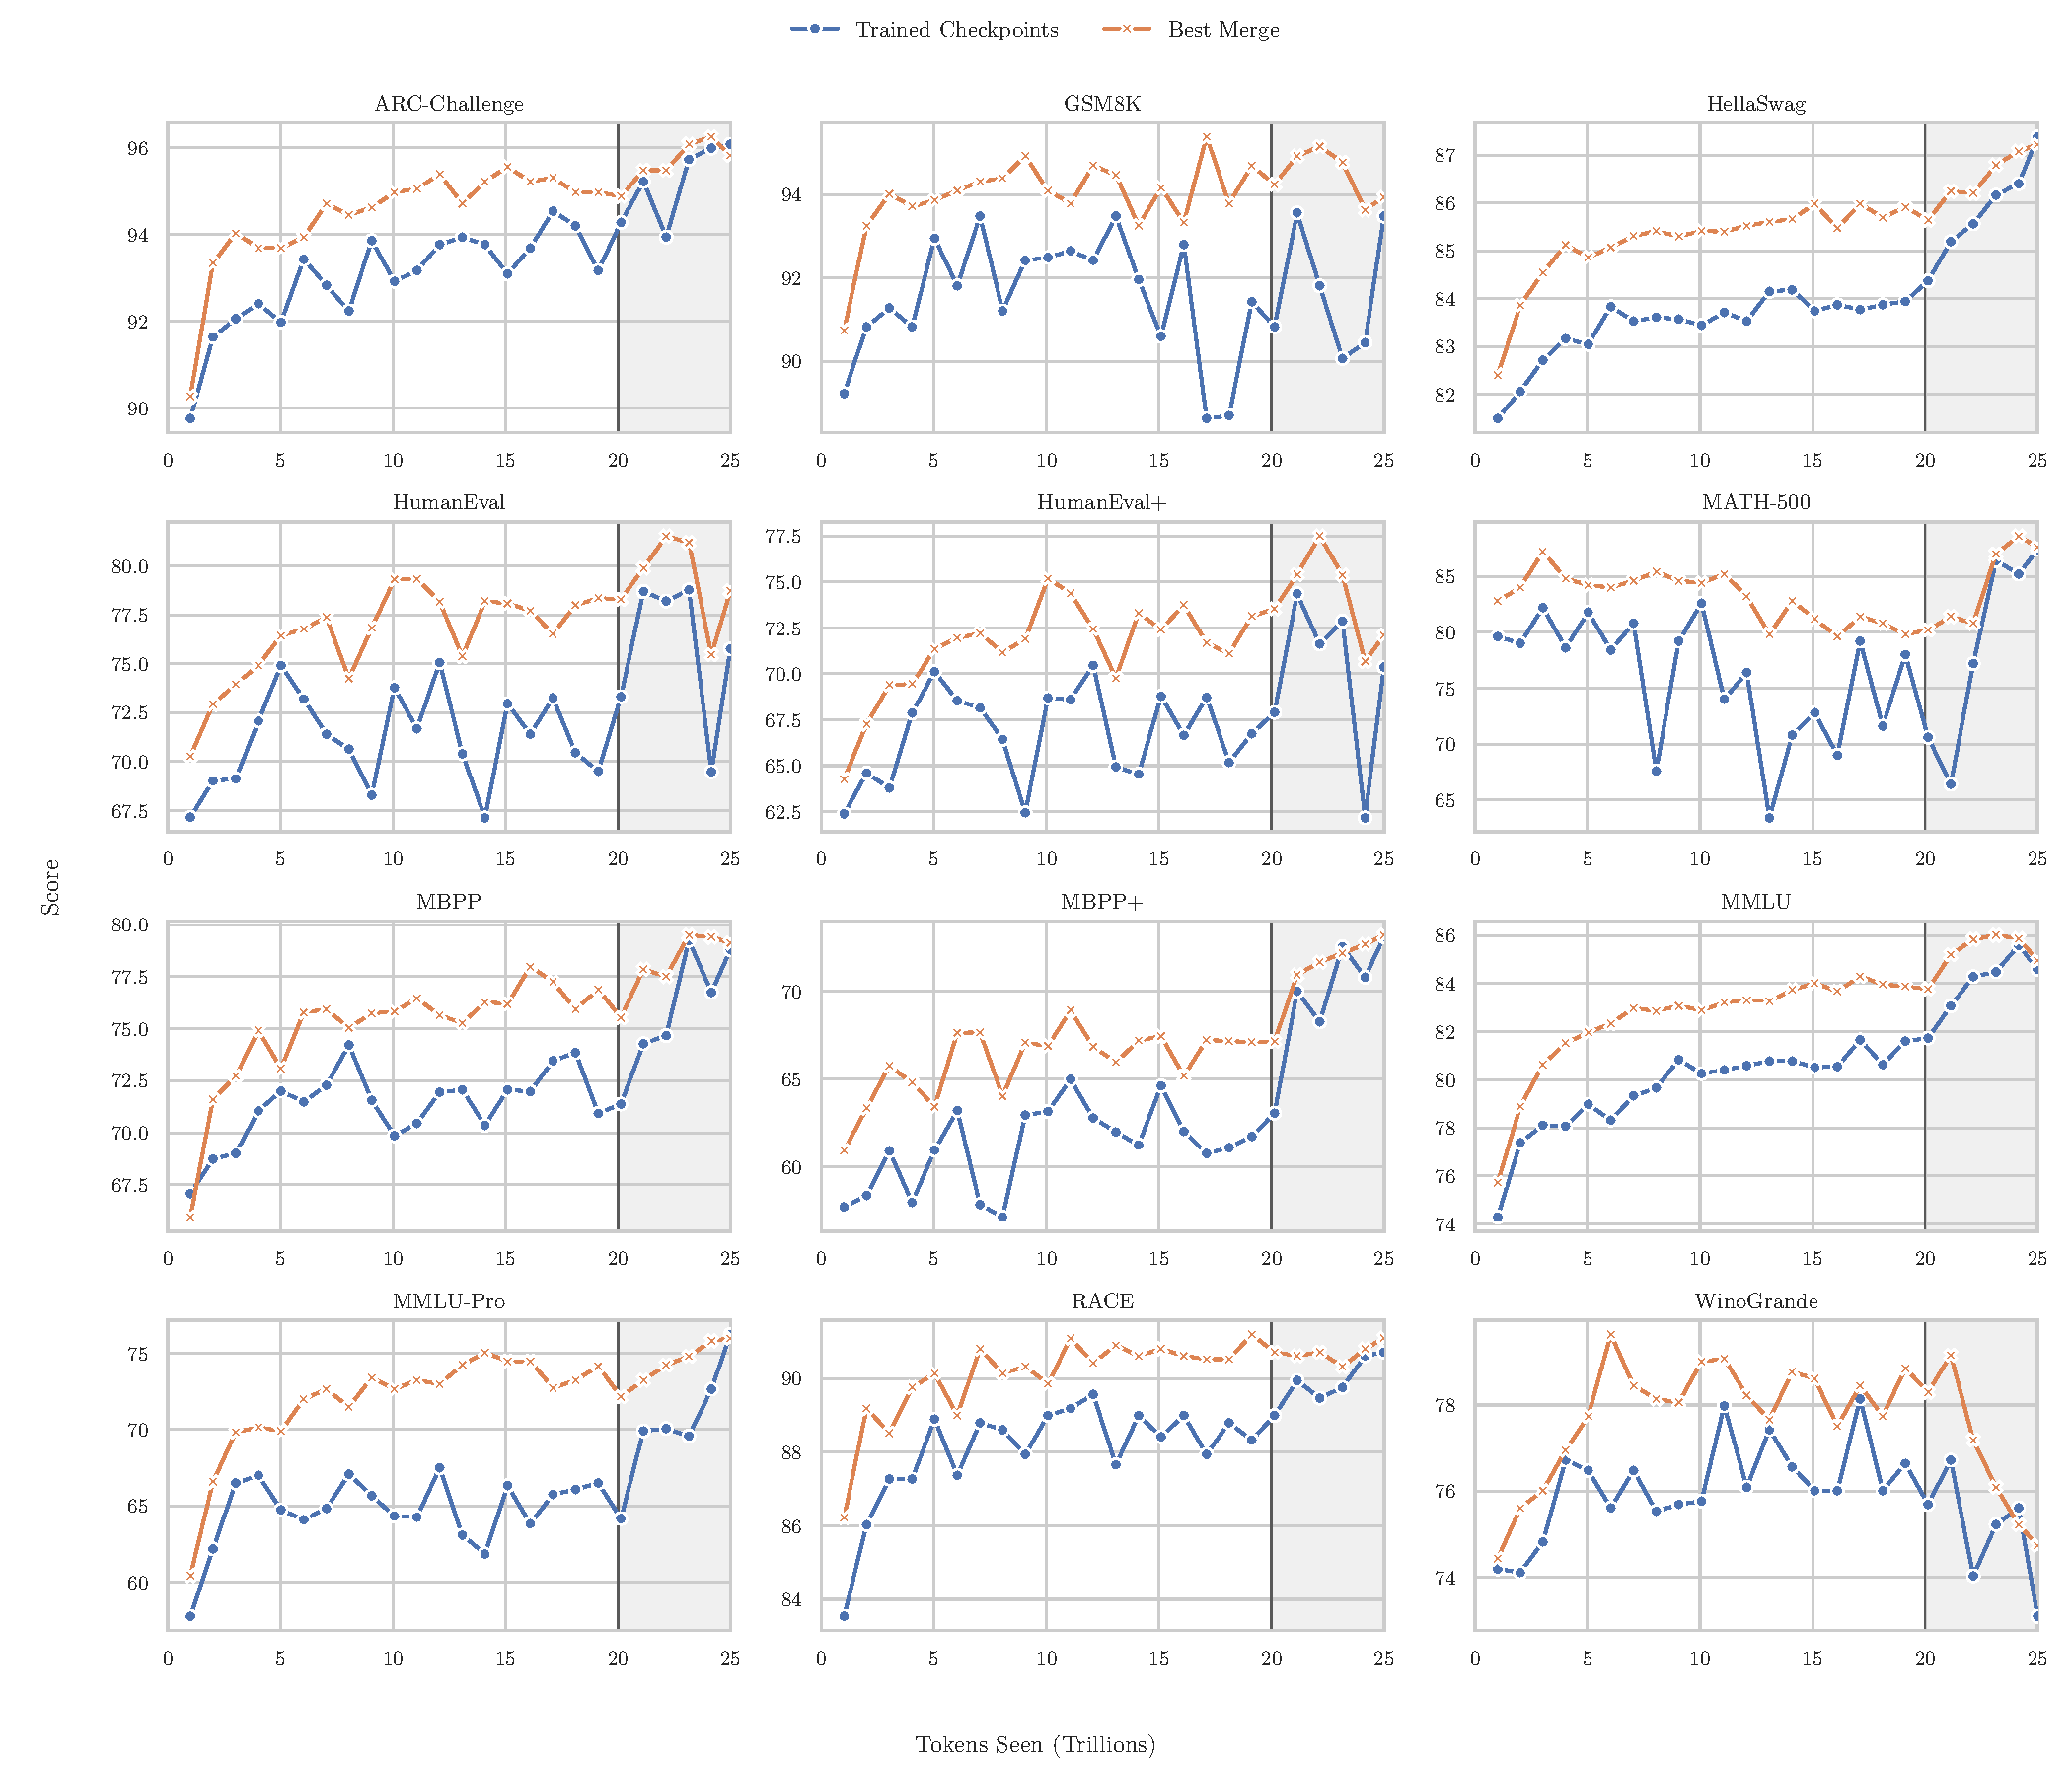
\includegraphics[width=\textwidth]{figures/per_benchmark.pdf}
    \caption{Per-benchmark accuracy for trained checkpoints versus the best offline checkpoint merge across the full 25T-token training run. The 12 benchmarks span general knowledge (MMLU-Pro, MMLU), code generation (HumanEval, HumanEval+, MBPP, MBPP+), mathematical reasoning (GSM8K, MATH-500), and commonsense understanding (RACE, ARC-Challenge, HellaSwag, WinoGrande). The shaded region indicates the LR decay phase.}
    \label{fig:per-benchmark}
\end{figure}

\section{FP4 Post Training Quantization (PTQ) Algorithm Details}

\subsection{PTQ Algorithm Ablation}
\label{sec:ptq-algorithm-ablation}
This section shows evaluation accuracy for various PTQ algorithms. In these experiments, all linear layers except the final classification layer and attention linear layers are quantized to NVFP4.

% \begin{table}[h]
% \centering
% \small
% \caption{PTQ Algorithm Ablation}
% \label{tab:ptq-algorithm-ablation}
% \resizebox{\textwidth}{!}{%
% \begin{tabular}{|p{3.8cm}|p{5.2cm}|c|c|c|c|}
% \hline
% \textbf{Algorithm} & \textbf{Details} & \textbf{MMLU-Pro} & \textbf{GPQA} & \textbf{LiveCodeBench} & \textbf{AA-LCR} \\
% \hline
% BF16 & --- & 83.49 & 79.92 & 72.907 & 53.00 \\
% \hline
% Default NVFP4 PTQ (Baseline algorithm) & Static per-tensor scales are computed using max-value calibration; per-block scales are computed dynamically from block maximum values. & 82.99 & 79.29 & 70.18 & 55.50 \\
% \hline
% Weight per-block scales minimizing MSE + Default NVFP4 PTQ & Weight per-block scales are swept to minimize per-block MSE. & 83.31 & 79.92 & 71.37 & 56.75 \\
% \hline
% Weight per-block scales to minimize output MSE + Default NVFP4 PTQ & Weight per-block scales are swept independently to minimize output MSE. & 83.05 & 78.98 & 71.00 & 57.06 \\
% \hline
% GPTQ + Default NVFP4 PTQ & GPTQ is used for weight quantization. & 83.11 & 80.05 & 69.79 & 57.87 \\
% \hline
% \end{tabular}%
% }
% \end{table}


\begin{table}[h]
\centering
\caption{PTQ Algorithm Ablation}
\label{tab:ptq-algorithm-ablation}
\resizebox{\textwidth}{!}{%
\begin{tabular}{l p{6cm} c c c c}
\toprule
\textbf{Algorithm} & \textbf{Details} & \textbf{MMLU-Pro} & \textbf{GPQA} & \textbf{LiveCodeBench} & \textbf{AA-LCR} \\
\midrule
BF16 & --- & 83.49 & 79.92 & 72.907 & 53.00 \\
\midrule
Default NVFP4 PTQ (Baseline algorithm) & Static per-tensor scales are computed using max-value calibration; per-block scales are computed dynamically from block maximum values. & 82.99 & 79.29 & 70.18 & 55.50 \\
\midrule
Weight per-block scales minimizing MSE & Weight per-block scales are swept to minimize per-block MSE. & 83.31 & 79.92 & 71.37 & 56.75 \\
\midrule
Weight per-block scales to minimize output MSE & Weight per-block scales are swept independently to minimize GEMM output MSE. & 83.05 & 78.98 & 71.00 & 57.06 \\
\midrule
GPTQ & GPTQ~\citep{gptq} is used for weight quantization. & 83.11 & 80.05 & 69.79 & 57.87 \\
\bottomrule
\end{tabular}%
}
\end{table}

\subsection{AutoQuantize Algorithm}
\label{sec:autoquantize-details}

The sensitivity of each operation is measured at its immediate (or closest available) output using a second-order metric:
\[
S(\mathrm{Op}_i, Q_{i,f}) = \left(Y_i^{\mathrm{bf16}} - Y_i^{Q_{i,f}}\right)^\top H_i \left(Y_i^{\mathrm{bf16}} - Y_i^{Q_{i,f}}\right)
\]
where $i$ indexes operators, $Q_{i,f}$ denotes the quantized operator under format choice $f$ for operator $i$, and $H_i$ is the local Hessian approximation at the selected measurement point. The measurement point $Y_i$ can be any location where quantization error is compared against BF16; for linear layers, we use the linear-layer output.

Computing the full Hessian is expensive, so we use a diagonal Hessian approximation and estimate it empirically with the diagonal Fisher information matrix. Define
\[
\Delta Y_i = Y_i^{\mathrm{bf16}} - Y_i^{Q_{i,f}} \qquad g_i = \nabla_{Y_i} \mathcal{L}
\]
where $Y_i, g_i \in \mathbb{R}^{d}$. The resulting sensitivity proxy is
\[
S(\mathrm{Op}_i, Q_{i,f}) \approx \sum_{k=1}^{d} (\Delta Y_{i,k})^2 (g_{i,k})^2
\]

The performance cost is defined as:
\[
C(\mathrm{Op}_i, Q_{i,f}) = \mathrm{FLOPs}(\mathrm{Op}_i, Q_{i,f})
\]

AutoQuantize then solves the constrained optimization:
\[
\min_{\{f\}} \sum_i S(\mathrm{Op}_i, Q_{i,f}) \quad \mathrm{s.t.} \quad \sum_i C(\mathrm{Op}_i, Q_{i,f}) \leq B
\]
where $Q_{i,f}$ is the chosen format for operator $i$, and $B$ is the total deployment cost budget.

\subsubsection{Deployment-Restriction-Aware Search}

\paragraph{1) Linear layer fusion.}
Inference runtimes often fuse linear operators, which imposes a shared quantization format across the fused group. This fusion constraint is applied within each layer: only that layer's Q, K, and V projections are fused and required to share one quantization format. For the fused QKV projection, we model the group as one decision variable and aggregate sensitivity and cost as
\[
\begin{aligned}
S(\mathrm{Op}_{\mathrm{qkv}}, Q_{\mathrm{qkv},f}) &= S(\mathrm{Op}_{\mathrm{q}}, Q_{\mathrm{qkv},f}) + S(\mathrm{Op}_{\mathrm{k}}, Q_{\mathrm{qkv},f}) + S(\mathrm{Op}_{\mathrm{v}}, Q_{\mathrm{qkv},f}) \\
C(\mathrm{Op}_{\mathrm{qkv}}, Q_{\mathrm{qkv},f}) &= C(\mathrm{Op}_{\mathrm{q}}, Q_{\mathrm{qkv},f}) + C(\mathrm{Op}_{\mathrm{k}}, Q_{\mathrm{qkv},f}) + C(\mathrm{Op}_{\mathrm{v}}, Q_{\mathrm{qkv},f})
\end{aligned}
\]
This formulation is valid under our second-order sensitivity approximation: when the fused operator enforces one shared format but preserves additive branch contributions, the quadratic sensitivity term for the fused output remains additive across Q, K, and V.

\paragraph{2) MoE layer constraints.}
vLLM and TensorRT-LLM quantized MoE APIs require all sparse experts in a constrained MoE group to share one quantization format. This shared-format restriction is also applied within each MoE layer: only sparse experts inside the same layer are coupled. In Nemotron 3 Super, each sparse expert contains \texttt{up\_proj} and \texttt{down\_proj}, and these sparse-expert projections must therefore be assigned jointly. We formulate the sparse-expert set as one operator-level decision,
\[
\mathrm{Op}_{\mathrm{moe}} = \bigcup_{e \in \mathcal{E}} \{\mathrm{Op}_{e,\mathrm{up\_proj}}, \mathrm{Op}_{e,\mathrm{down\_proj}}\}
\]
where \(\mathrm{moe}\) denotes the MoE sparse-expert group (all coupled sparse-expert \texttt{up\_proj}/\texttt{down\_proj} operators within one MoE layer).
We measure sensitivity at the MoE block output so that the metric captures the combined contribution from all sparse experts,
\[
S(\mathrm{Op}_{\mathrm{moe}}, Q_{\mathrm{moe},f}) = \left(Y_{\mathrm{moe}}^{\mathrm{bf16}} - Y_{\mathrm{moe}}^{Q_{\mathrm{moe},f}}\right)^\top H_{\mathrm{moe}} \left(Y_{\mathrm{moe}}^{\mathrm{bf16}} - Y_{\mathrm{moe}}^{Q_{\mathrm{moe},f}}\right)
\]
and define the deployment cost as the sum over sparse experts,
\[
C(\mathrm{Op}_{\mathrm{moe}}, Q_{\mathrm{moe},f}) = \sum_{e \in \mathcal{E}} \left(C(\mathrm{Op}_{e,\mathrm{up\_proj}}, Q_{\mathrm{moe},f}) + C(\mathrm{Op}_{e,\mathrm{down\_proj}}, Q_{\mathrm{moe},f})\right)
\]
Other linear layers in the MoE block, such as latent projection layers and shared experts, are not part of this sparse-expert coupling constraint and can be assigned different quantization formats.